\section{Introduction\label{sec:intro}}

\subsection{Goals}

The LSST is a facility whose primary mission is to acquire, process, and
make available the data\footnote{This includes the raw and processed calibration and engineering data, in addition to the data collected by the science sensors. Because much of LSST science will be systematics limited, access to engineering data will enable a better understanding and correction of subtle instrumental and/or environmental effects.} collected by its telescope and camera, as well as enable ``next-to-the-data'' creation of added-value (Level 3) data products
(see the \SRD and the \LSR).

This document describes the vision for the services to be put into place to
fulfill the ``\emph{making available}'' and ``\emph{Level 3} creation``
aspects of LSST's mission. Its aim is to present a high-level
description of the data access and analysis services provided at the
LSST Data Access Centers. It should be read in conjunction with the
LSST Data Products Definition Document (\DPDD), which provides the high-level
description of LSST data products.

\subsection{LSST Science Platform Overview}

\begin{figure}
\centering
\scalebox{0.4}{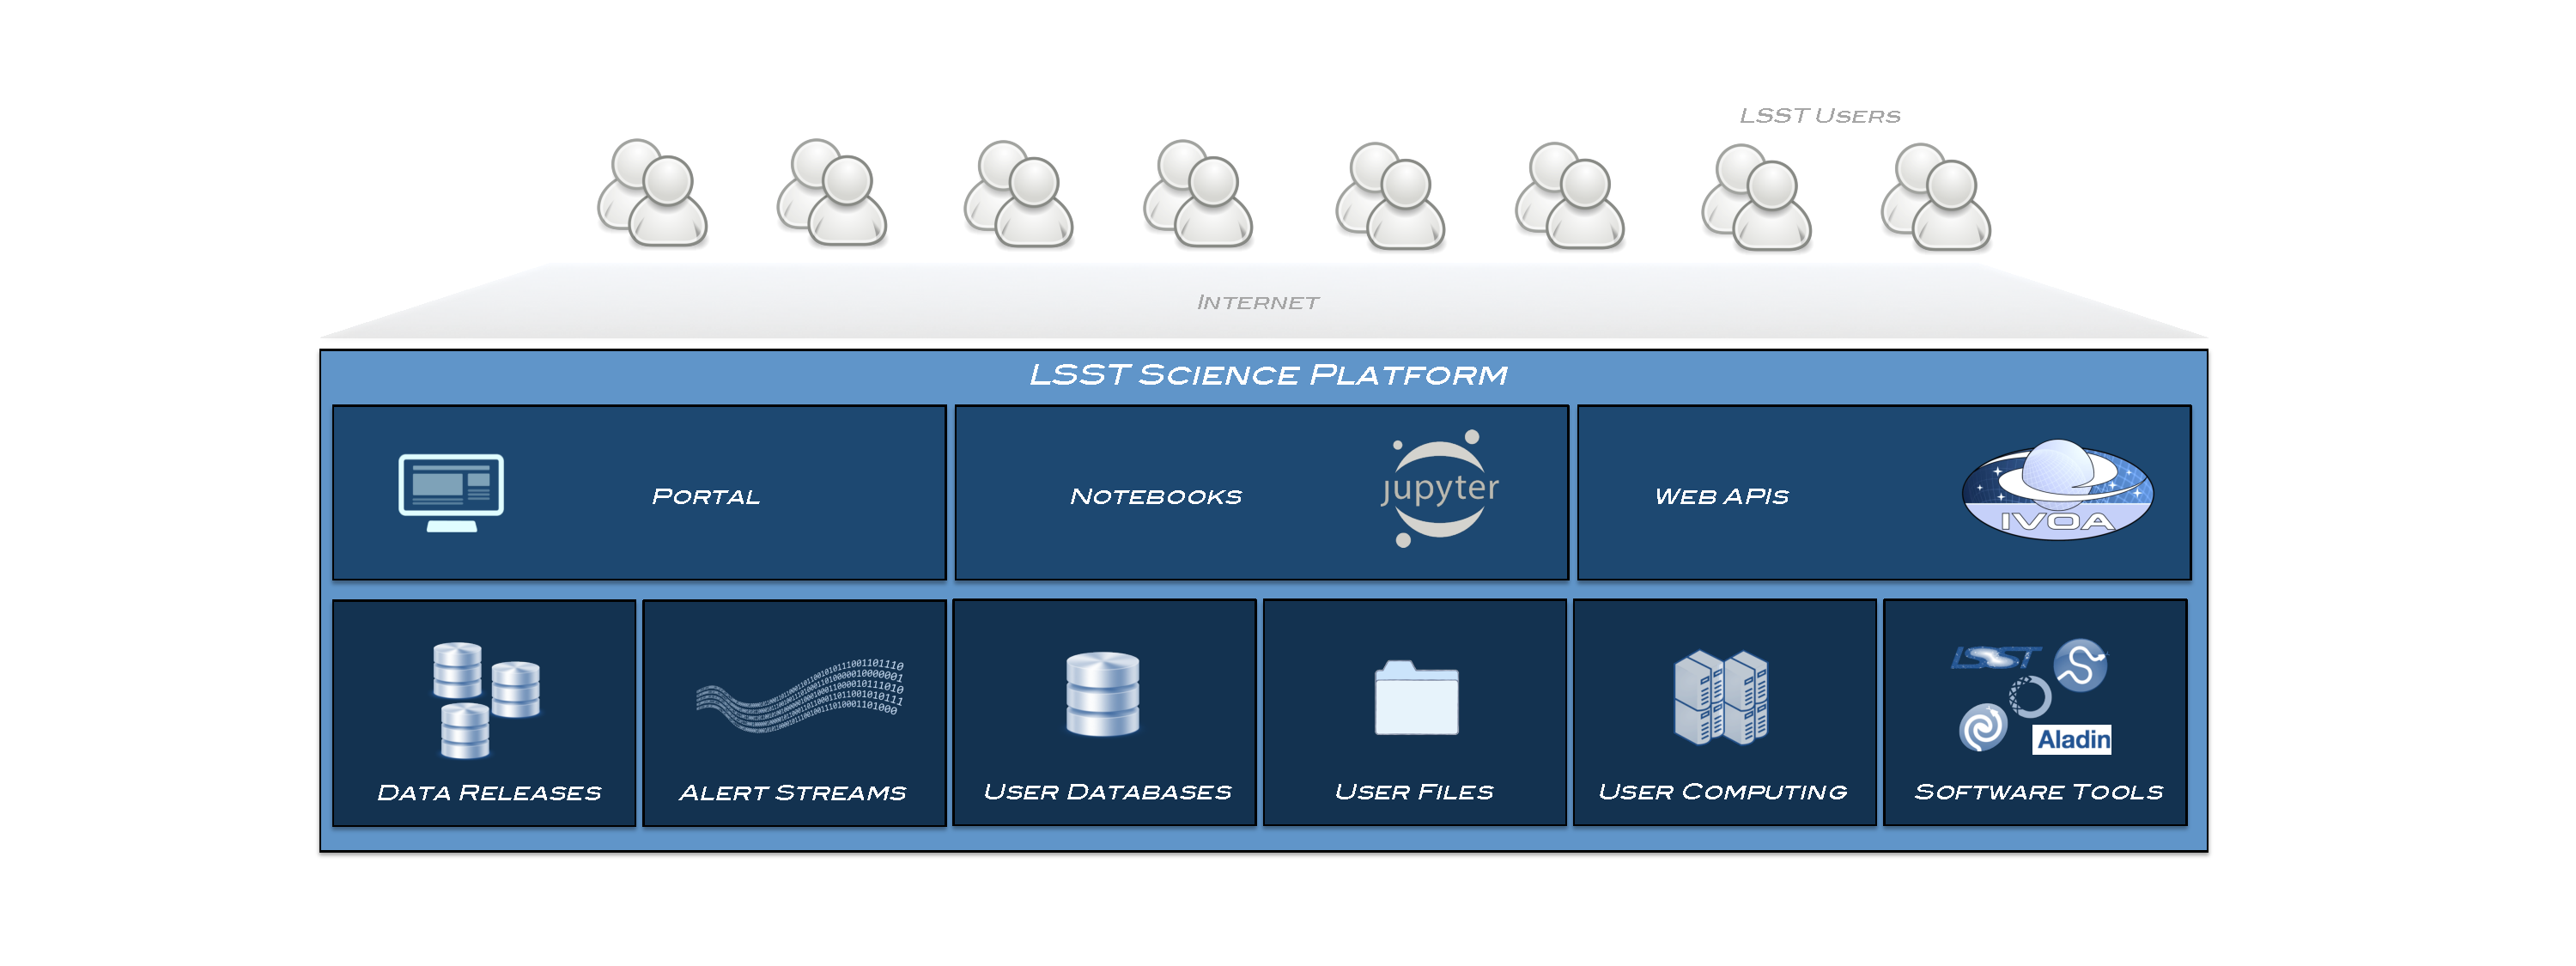
\includegraphics[trim={5cm 0.5cm 3cm 0.5cm},clip,page=1]{images/fig-lsst-science-platform-extended}}
\caption{
A high-level, layered, view of the LSST Science Platform.  The LSST data
will be exposed to the users through the web Portal, the Jupyter Notebook
interface, and machine-accessible Web APIs.  The web Portal component will
provide the essential data access and visualization services common to
present day archives.  The Notebook component, based on the Jupyter family
of technologies (JupyterHub and JupyterLab) will allow for more
sophisticated next-to-the-data analysis.  These user-visible services will
provide acces to the underlying core LSST data sets -- the data releases and
alert streams -- and be supported by the user Database, File Storage,
Computing, and Software Tools components.  Together, they will enable the
users to access, sub-select, analyze, and perform added-value processing of
all flavors of LSST Data Products (see text for detail).
\label{fig:layeredLSP}}
\end{figure}

We define the \textbf{LSST Science Platform as a set of web applications and services
made available to the scientific community to access, visualize, subset, and
perform next-to-the-data analysis of the LSST data set}. It represents the integrated
set of services that will be offered to LSST users.

The platform exposes the LSST data
and services to the user through three primary user-facing ``\textit{aspects}'' -- the web \textbf{Portal},
the \textbf{JupyterLab} analysis environment, and a machine-accessible \textbf{Web API} interface. These aspects provide three different ways to access the data sets and analysis services provided in the LSST Data Access Centers (Figure~\ref{fig:layeredLSP}).

The first, \textbf{Portal}, aspect is a web portal designed to provide the essential data
access and visualization services through a simple-to-use website.  It will
enable browsing and visualization of the available datasets in ways the
users are accustomed to at archives such as IRSA, MAST, or the SDSS archive.
We describe it in more detail in \secref{sec:portal}.

The second, \textbf{JupyterLab}, aspect will provide a Jupyter Notebook-like interface, and
is geared towards enabling next-to-the-data analysis. The user experience will
be nearly identical to working with Jupyter notebooks locally, except that computation
and analysis will occur with resources provided at the LSST Data Access Center.  This is an
implementation of the “bringing computation to the data” paradigm: rather
than imposing the burden of downloading, storing, and processing (potentially large)
subsets of LSST data at their home institutions, we will enable our users to
bring their codes and perform their analysis at the LSST DAC.
This reduces the barrier to entry and shortens the path to science for
the LSST science community. We describe it in more detail in \secref{sec:jupyter}.

The third, \textbf{Web API}, aspect of the LSST Science Platform will expose the
services offered by the LSST Data Access Centers to other software tools and
services using commonly accepted protocols. For example, industry-standard
protocols such as WebDAV may be used to expose file data, or Virtual Observatory
protocols for access to catalogs or images (TAP and SIAP, respectively). This interface will open the
possibility for remote access and analysis of the LSST  data set using
applications that the users are already comfortable with (eg., such as TOPCAT
or libraries like Astropy). Furthermore, the offered APIs will allow for federation
with other astronomical archives, bringing added value to the LSST dataset.
We describe it in more detail in \secref{sec:apis}.

Enabling these user-facing aspects is a set of backend services. The Data Releases will be organized as catalogs kept in relational database management systems, as well as repositories of files. The alert distribution system will facilitate the distribution of Alert Streams to community brokers and end-users (see the \DPDD for details). These services will be complemented by additional User Database, File Storage, and Batch Computing services, as well as pre-installed Software Tools suite. They will provide the computational power, data storage, and analytics capabilities needed to enable LSST data analysis as well as the creation and federation of Level 3 products. We further describe these in \secref{sec:backend}.

Finally, the LSST Science Platform is being envisioned to enable and encourage
collaborative work.  The capabilities ranging from sharing of derived
datasets within smaller groups, collaborations, or with the broader LSST
community, to collaborative visualization and editing capabilities expected
to become available within the JupyterLab ecosystem (\secref{sec:collab}).